% !TeX spellcheck = en_US
\section{Problem 2}

We are asked to write a Python program that implements steepest descent algorithm for the 1-$S^1$-1 RBF network.
The input function that we want to approximate is 
\[
g(p) = 1 + \sin\left(p\pi/8\right), \quad \text{for} \ p \in \left[-4,4\right]
\]

We select 30 data randomly from that interval and all parameters are initialized as small numbers using \verb|numpy.random.randn| function. It returns a number at the exact specification as needed.

\begin{figure}[htbp]
	\centering
	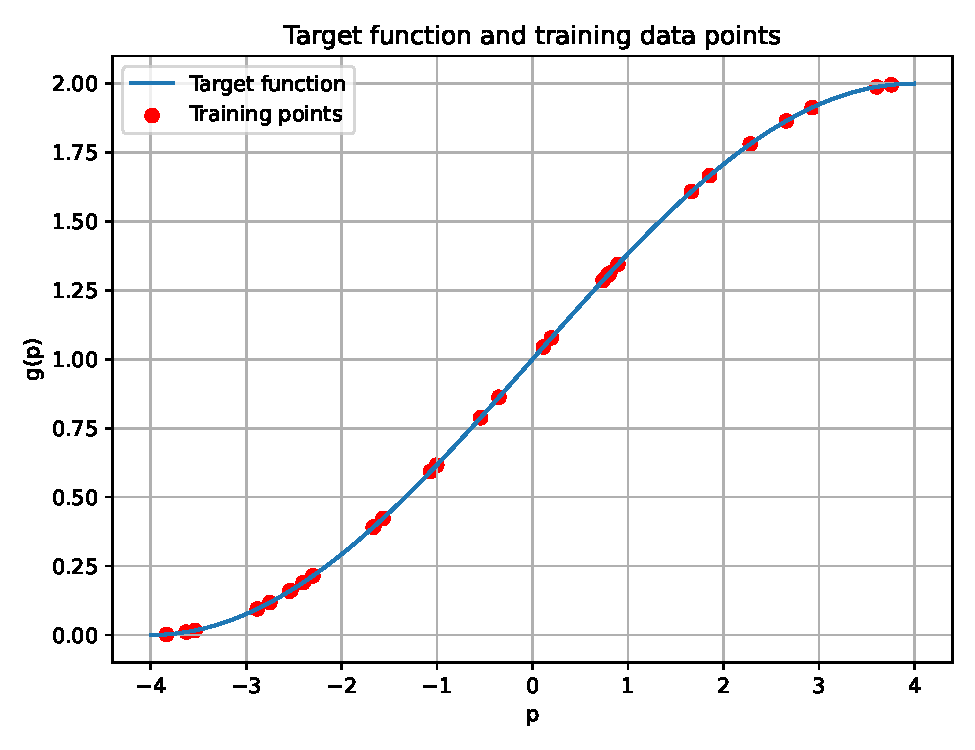
\includegraphics[width=0.6\linewidth]{../Problem 2/prob2_targetFunc_dataPoints.pdf}
	\caption{Input function in the specified area and the randomly assigned train data points.}
\end{figure}

For the randomly assigned data points, we added a custom seed number using in order for the results to be comparable but still use randomness.
